\documentclass[11pt,a4paper]{article}
\usepackage[T1]{fontenc}
\usepackage[utf8]{inputenc}
\usepackage[polish]{babel}
\usepackage{lmodern}
\usepackage{geometry}
\usepackage{booktabs}
\usepackage{siunitx}
\usepackage{hyperref}
\usepackage{graphicx}
\usepackage{float}
\usepackage{caption}
\usepackage{array}

\geometry{margin=2.5cm}
\sisetup{round-mode=places,round-precision=4}

\title{Projekt 1: easyAI -- Nim i Nimby}
\author{Mikołaj Dudkiewicz \and Eliza Petrycka}
\date{\today}

\begin{document}
\hypersetup{pageanchor=false}
\begin{titlepage}
    \centering
    {\large AGH\par}
    \vspace{0.4cm}
    {\large WEAIiIB ISI\par}
    \vspace{2.5cm}
    {\LARGE \textbf{Projekt 1: easyAI -- Nim i Nimby}\par}
    \vspace{1.2cm}
    {\large Przedmiot: Inteligencja obliczeniowa\par}
    \vspace{1.8cm}
    \begin{tabular}{>{\raggedright\arraybackslash}p{0.35\textwidth} p{0.55\textwidth}}
        Autorzy: & Mikołaj Dudkiewicz \\
                 & Eliza Petrycka \\
        Grupa:   & [6] \\
    \end{tabular}
    \vfill
    {\large \today\par}
\end{titlepage}

\tableofcontents
\newpage
\hypersetup{pageanchor=true}
\pagenumbering{arabic}

\section{Opis zadania i gry}
W ramach laboratorium zrealizowano wszystkie punkty z pliku \texttt{EasyAI.pdf}.
Wybrana gra probabilistyczna to \textbf{Nimby}. Zakres obejmuje:
\begin{itemize}
    \item implementacje wariantu probabilistycznego gry,
    \item turnieje AI vs AI z kontrola gracza rozpoczynajacego,
    \item porownanie algorytmow Negamax (z i bez odciecia alfa-beta),
    \item pomiar czasu podejmowania decyzji,
    \item implementacje wariantu expecti-minimax z odcieciem alfa-beta.
\end{itemize}

Gra bazowa to klasyczny Nim (wariant misere): gracz zabierajacy ostatni element przegrywa.
Stan poczatkowy w eksperymentach: trzy stosy \((3,4,5)\). Wariant Nimby wprowadza
szum wykonania: dla ruchu ``zabierz $k$'' (gdy $k>1$), z prawdopodobienstwem $0.1$
wykonywane jest ``zabierz $k-1$''.

\section{Implementacja}
Kod znajduje sie w pliku \texttt{lab\_01/nimby\_experiments.py}.
Zaimplementowano:
\begin{itemize}
    \item klase \texttt{NimbyGame} (deterministyczny Nim i probabilistyczny Nimby przez parametr \texttt{error\_probability}),
    \item \texttt{NegamaxNoAB} -- Negamax bez odciecia alfa-beta,
    \item \texttt{ExpectiNegamaxAB} -- wariant expecti-minimax z odcieciem alfa-beta,
    \item \texttt{TimedAIPlayer} -- zliczanie czasu decyzji i liczby ruchow,
    \item runner eksperymentow zapisujacy wyniki do \texttt{lab\_01/results.json}.
\end{itemize}

\paragraph{Wazny aspekt implementacyjny.}
W srodowisku probabilistycznym nie mozna tracic spojnosci miedzy \texttt{make\_move}
a \texttt{unmake\_move}. Dlatego rzeczywista liczba zabranych elementow jest zapisywana
na stosie historii i cofana 1:1. Dla expecti-minimax zamiast losowania uzyto jawnych
wezlow szansy (normalny ruch vs ``slip'') i wartosci oczekiwanej:
\[
E = (1-p)\,V_{\text{normal}} + p\,V_{\text{slip}}, \quad p=0.1.
\]

Wykresy do raportu sa generowane automatycznie przez skrypt
\texttt{lab\_01/generate\_plots.py} na podstawie \texttt{lab\_01/results.json}.

\section{Metodologia eksperymentow}
Wszystkie testy uruchomiono skryptem:
\begin{center}
\texttt{uv run python lab\_01/nimby\_experiments.py}
\end{center}

Wspolne ustawienia:
\begin{itemize}
    \item naprzemienne rozpoczynanie partii (eliminacja biasu pierwszego ruchu),
    \item limit 200 polruchow na partie (w praktyce brak remisow),
    \item te same stany poczatkowe i kontrola ziaren losowosci po numerze partii.
\end{itemize}

\section{Wyniki -- zadania na 4 punkty}
Porownano dwa ustawienia glebokosci Negamax: \texttt{depth=4} i \texttt{depth=6},
osobno dla Nim (deterministyczny) i Nimby (probabilistyczny).

\begin{table}[h!]
\centering
\caption{NegamaxAB depth 4 vs depth 6 (200 partii)}
\begin{tabular}{lrrrr}
\toprule
Wariant & Wygrane d4 & Wygrane d6 & Remisy & Sredni czas ruchu [ms] d4 : d6 \\
\midrule
Nim (det.) & 0 & 200 & 0 & 0.7146 : 5.4021 \\
Nimby (prob.) & 104 & 96 & 0 & 0.8147 : 6.0359 \\
\bottomrule
\end{tabular}
\end{table}

\paragraph{Komentarz.}
W wariancie deterministycznym glebsze przeszukiwanie dominuje calkowicie.
W wariancie probabilistycznym roznica glebokosci przestaje byc monotonicznie korzystna:
przypadkowosc wykonania ruchu zaburza planowanie klasycznego Negamax.

\begin{figure}[H]
\centering
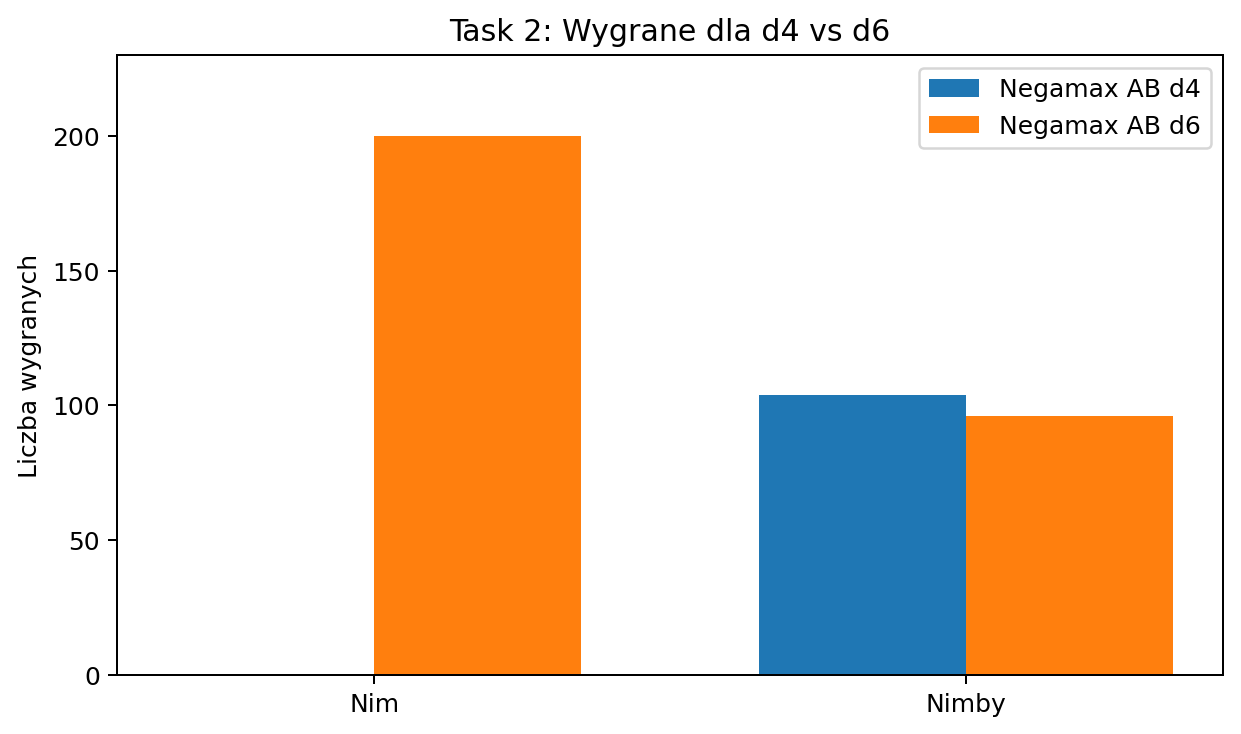
\includegraphics[width=0.82\textwidth]{figures/task2_wins.png}
\caption{Task 2: liczba wygranych dla NegamaxAB d4 i d6.}
\label{fig:task2wins}
\end{figure}

\section{Wyniki -- zadania na 6 punktow}
Wykonano porownanie Negamax z i bez odciecia alfa-beta, dla dwoch glebokosci (4, 6)
i dla obu wariantow gry.

\begin{table}[h!]
\centering
\caption{Negamax z/bez alfa-beta (100 partii na kazde starcie)}
\begin{tabular}{llrrrr}
\toprule
Wariant & Starcie & Wygrane A & Wygrane B & Czas A [s] & Czas B [s] \\
\midrule
Nim & AB d4 vs NoAB d4 & 50 & 50 & 0.3694 & 2.1376 \\
Nim & AB d6 vs NoAB d6 & 50 & 50 & 2.3406 & 23.1431 \\
Nimby & AB d4 vs NoAB d4 & 59 & 41 & 0.3349 & 2.3374 \\
Nimby & AB d6 vs NoAB d6 & 51 & 49 & 1.8052 & 25.6892 \\
\bottomrule
\end{tabular}
\end{table}

\paragraph{Wnioski.}
Decyzje strategiczne AB i NoAB sa porownywalne (w Nim idealnie identyczne),
ale wydajnosc czasowa AB jest wielokrotnie lepsza. Dla \texttt{depth=6}
bez odciecia koszt obliczen jest rzedu $10\times$ wiekszy.

\begin{figure}[H]
\centering
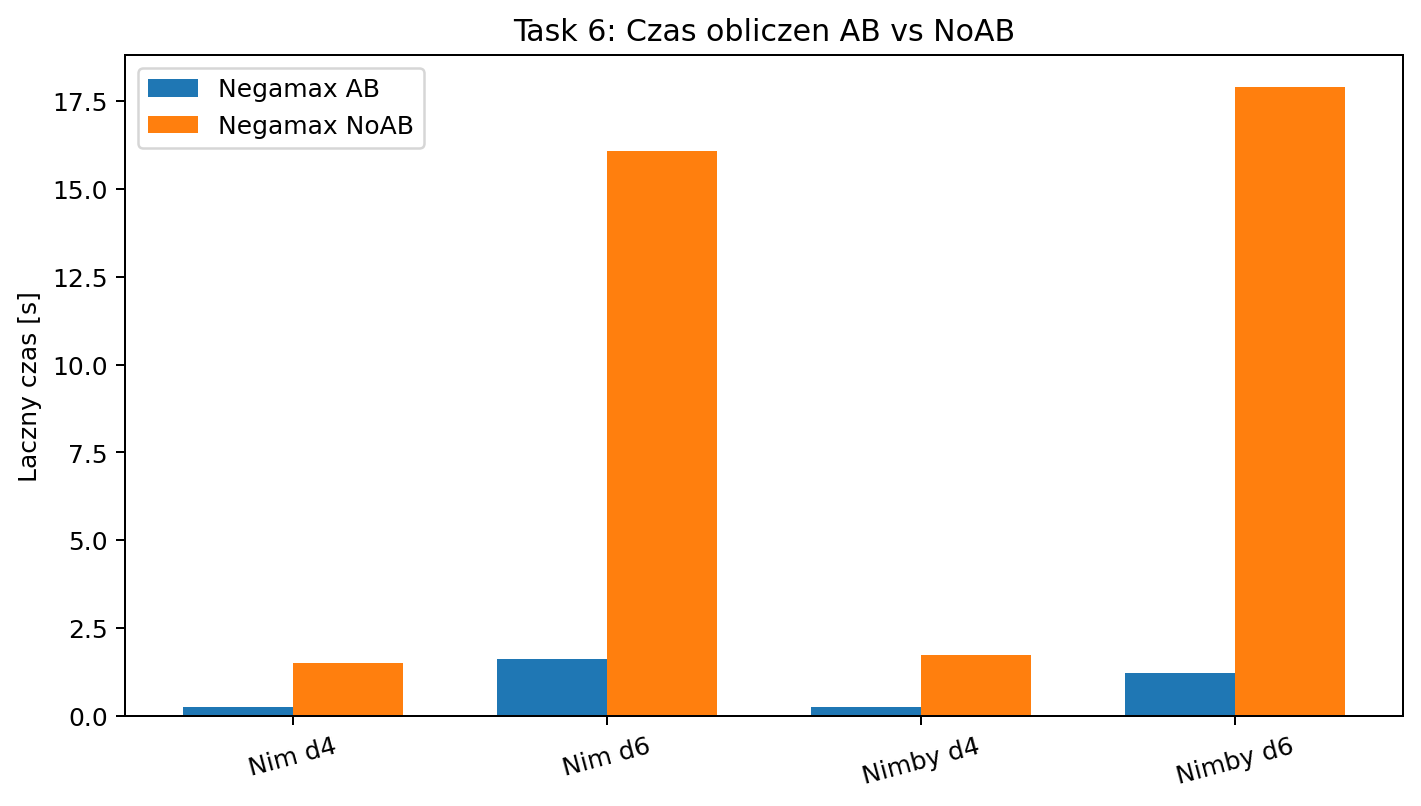
\includegraphics[width=0.9\textwidth]{figures/task6_times.png}
\caption{Task 6: porownanie lacznego czasu obliczen AB vs NoAB.}
\label{fig:task6times}
\end{figure}

\section{Wyniki -- zadania na 8 punktow}
Zaimplementowano expecti-minimax z odcieciem alfa-beta i porownano z klasycznym
NegamaxAB w Nimby.

\begin{table}[h!]
\centering
\caption{NegamaxAB vs ExpectiNegamaxAB (Nimby, 100 partii)}
\begin{tabular}{lrrrr}
\toprule
Starcie & Wygrane Negamax & Wygrane Expecti & Czas Negamax [s] & Czas Expecti [s] \\
\midrule
Depth 4 & 25 & 75 & 0.3544 & 0.9316 \\
Depth 6 & 23 & 77 & 2.1210 & 11.0509 \\
\bottomrule
\end{tabular}
\end{table}

\paragraph{Wnioski koncowe.}
Expecti-minimax wyraznie poprawia skutecznosc w grze probabilistycznej, bo modeluje
ryzyko bledu wykonania ruchu. Cena za te poprawe to wyzszy czas obliczen
(okolo $2.6\times$ dla depth 4 i ponad $5\times$ dla depth 6).

\begin{figure}[H]
\centering
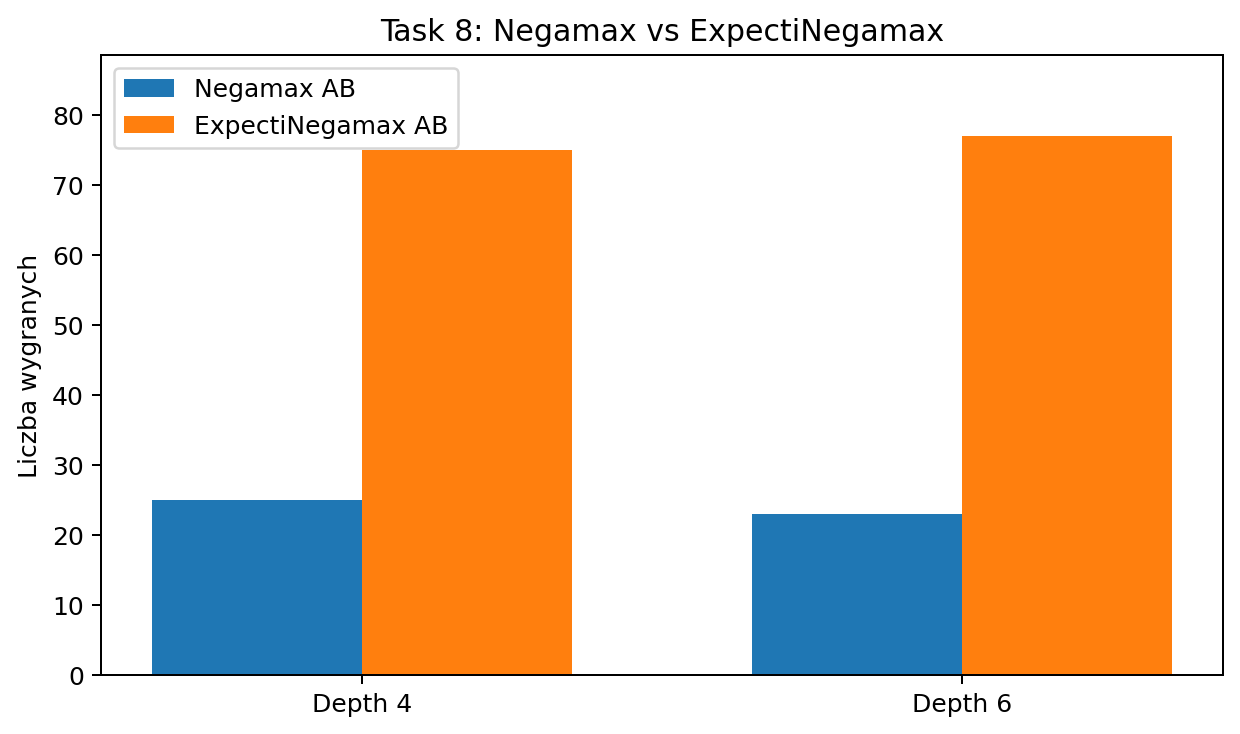
\includegraphics[width=0.82\textwidth]{figures/task8_wins.png}
\caption{Task 8: NegamaxAB kontra ExpectiNegamaxAB (Nimby).}
\label{fig:task8wins}
\end{figure}

\section{Napotkane problemy}
Glownym problemem byla zgodnosc logiki probabilistycznej z mechanizmem przeszukiwania
drzewa. Negamax zaklada spojnosc wykonania/cofania ruchu; przy naiwnej losowosci
w \texttt{make\_move} mozna latwo uszkodzic stan gry. Problem rozwiazano przez:
\begin{itemize}
    \item jawna rejestracje rzeczywiscie wykonanego ruchu,
    \item deterministyczne cofanie ruchow po historii,
    \item osobne modelowanie wezlow szansy w expecti-minimax.
\end{itemize}

\section{Reprodukowanie wynikow}
\begin{itemize}
    \item generowanie wykresow: \texttt{uv run python lab\_01/generate\_plots.py}
    \item uruchomienie: \texttt{uv run python lab\_01/nimby\_experiments.py}
    \item dane wyjsciowe: \texttt{lab\_01/results.json}
    \item raport: \texttt{lab\_01/report.tex}
\end{itemize}

\end{document}
